\section{Bead on a tilted wire}
\numberwithin{figure}{section}
In this section a bead with mass $m$ moves along a wire. As depicted in figure  \ref{fig:ex1beadeps}, the wire is rotated with an angle $\theta$ with respect to the vertical axis. The bead is connected to the bottom of the structure through a spring with spring constant $k$ and rest length $L_0$. The bead is also subject to a friction force $b\dot{x}$. 

\begin{figure}[htp]
\centering
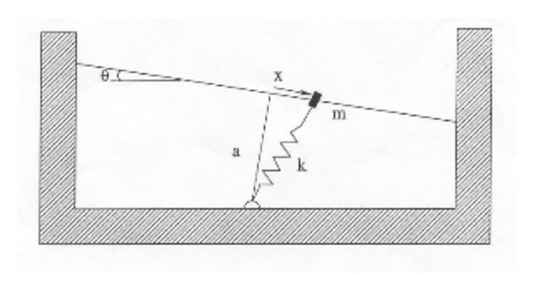
\includegraphics{img/ex1/bead.eps}
\caption{}
\label{fig:ex1beadeps}
\end{figure}

The system model represents Newton's equation for the motion of the bead on the wire
\begin{equation}
m\ddot{x}=mg\sin{\theta} -b\dot{x}-kx\left(1-\frac{L_0}{\sqrt{x^2+a^2}}\right)\label{eqn:newton2order}
\end{equation}
This system can be split up into a more useful form with variables $x$ and $\dot{x}$ and only first order derivatives
 \begin{align}
 \frac{dx}{dt}&=\dot{x}\label{eqn:dxdt}\\
 \frac{d\dot{x}}{dt}&=g\sin{\theta}-\frac{b}{m}\dot{x}-\frac{kx}{m}\left(1-\frac{L_0}{\sqrt{x^2+a^2}}\right)\label{eqn:ddotdt}
 \end{align}
 
 %% Theta=0
 
\subsection{The case $\theta=0$}\label{sec:ex1theta0}
In this section the system will be studied while the wire is vertical. This leads to a perfectly symmetrical system in $x$. 
\subsubsection{Fixed points and their stability}
In order to find the fixed points, a simple reasoning suffices. For the system of equations (\ref{eqn:dxdt})-(\ref{eqn:ddotdt}) to have a stationary solution at a point, both derivatives must be zero. From equation (\ref{eqn:dxdt}) it is clear that $\dot{x}$ must allways be zero. When this result is used in (\ref{eqn:ddotdt}), a condition on $x$ for $(x,0)$ to be a fixed point is obtained
\begin{align}
  \frac{d\dot{x}}{dt}=0&=-\frac{kx}{m}\left(1-\frac{L_0}{\sqrt{x^2+a^2}}\right)\label{eqn:ddotdt}
\end{align}
Thus either 
\begin{equation}
x=0 \mbox{\hspace{12pt}or\hspace{12pt}}x=\pm\sqrt{L_0^2-a^2}
\end{equation}
As is obvious from the formula, the two square roots will only exist if $a<L_0$. The stability of these fixed points can easily be derived when $m=0$. Equation\label{eqn:newton2order} then simplifies to the first order system
\begin{equation}
b\dot{x}=-kx\left(1-\frac{L_0}{\sqrt{x^2+a^2}}\right)\label{eqn:ex1firstorder}
\end{equation}
This derivative is plotted in figure \ref{fig:ex1stab} for both $a<L_0$ and $a>L_0$. From this figure it is clear that when $a<L_0$, the fixed points corresponding to the square roots are stable and the origin is unstable, and when $a>L_0$, the origin is stable. This is the typical behavior of a pitchfork bifurcation, as is shown in the bifurcation diagram in figure \ref{fig:ex1bif1}. The bifurcation diagram has free parameter $L_0$ and the pitchfork bifurcation occurs when $L_0=a$.
\begin{figure}[htp]
\centering
\subfloat[$a<L_0$]{
\includegraphics{img/ex1/stab1.eps}} \hspace{18pt}
\subfloat[$a>L_0$]{
\includegraphics{img/ex1/stab2.eps}}
\caption{}
\label{fig:ex1stab}
\end{figure}
\begin{figure}[htp]
\centering

\includegraphics{img/ex1/bif1.eps}
\caption{}
\label{fig:ex1bif1}
\end{figure}

The stability analysis is only valid when $m=0$. In order to determine for which relative values of $m$ this is a valid approximation, the system is first made dimensionless
\begin{equation}
\frac{m\ddot{x}}{ak}= -\frac{b\dot{x}}{ak}-\frac{x}{a}\left(1-\frac{L_0}{\sqrt{x^2+a^2}}\right)
\end{equation}
From this equation it is clear that the inertia term can only be neglected with respect to the other terms when $m<<b$, when the inertia is very small relative to the friction force.
\subsubsection{Comparison of the full system with its first order approximation}
For ease of use, the system is transformed to a simpler form
\begin{align}
\frac{\delta u}{\delta \tau} &= v \\
\frac{\delta v}{\delta \tau} &= -\frac{1}{\epsilon} [v+(1-\frac{R}{\sqrt{1+u^2}})u]
\end{align}
with 
\begin{equation}\label{eqn:ex1transfers}
R=\frac{L_0}{a}, u=\frac{x(t)}{a},v=\frac{\alpha \dot{x}(t)}{a},\epsilon=\frac{km}{b^2},\tau=\frac{t}{\alpha}\mbox{\hspace{4pt}and\hspace{4pt}} \alpha=\frac{b}{k}
\end{equation} 
When neglecting the inertia term as in (\ref{eqn:ex1firstorder}), a simplified first order system is obtained
\begin{equation}
\frac{\delta u}{\delta \tau}=(1-\frac{R}{\sqrt{1+u^2}})u
\end{equation}
The behavior of this first order approximation will be compared with the full system for $R=0.6463$. For this value of $R$ only the origin is stable. The parameter $\epsilon$ is varied for different starting values, and the two systems are then simulated until this equilibrium sets in. The results are shown in figure \ref{fig:ex1epsilon}. The bold curves are from the simulated first order system. The curves for the full system are shown for $\epsilon \in [0,0.5,1,2]$. As is obvious from the model equations, the two systems are equal when $\epsilon=0$. When $\epsilon$ grows, the behavior of the full system will distantiate from that of the first order approximation. The stable equilibrium is still reached, but the system has an overshoot that is not possible in first order systems.
\begin{figure}[htp]
\centering

\includegraphics{img/ex1/epsilon.eps}
\caption{}
\label{fig:ex1epsilon}
\end{figure}

A problem that is not yet considered is that of the initial value. For the full system, an initial position and velocity are required. In figure \ref{fig:ex1epsilon} this initial velocity is taken to be zero. However, the initial velocity of the first order system is determined by the equations. The initial velocity of the full system can be chosen according to this first order system. The results are shown in figure \ref{fig:epsilon2}. The solutions now start with the same velocity and their behavior is comparable for the first second, but aftwerwards the overshoot shows again and the solutions start to distantiate for growing $\epsilon$.
\begin{figure}[H]
\centering

\includegraphics{img/ex1/epsilon2.eps}
\caption{}
\label{fig:epsilon2}
\end{figure}

%% The case theta !=0
\subsection{The case $\theta \ne 0$}\label{sec:ex1thetane0}
The equations from section \ref{sec:ex1theta0} now gain a term depending on $\sin{\theta}$. When keeping the change of variables of (\ref{eqn:ex1transfers}) and adding $h=mg\sin{\theta}/ak$, the equilibrium equation becomes
\begin{equation}\label{eqn:ex1eqbreq}
1-\frac{h}{u}=\frac{R}{\sqrt{1+u^2}}
\end{equation}
which is equal to the equilibrium equation for $\theta=0$ except for the term in $h$. A graphical interpretation is given in figure \ref{fig:graphR}. In this figure $uR/\sqrt{1+u^2}-u+h$ is plotted as a function of $u$ for $h=0$ (bold curve) and $h=\pm0.1$ (striped curves). Where the graph intersects the x-axis an equilibrium is found. When interpreting the equilibrium equation in this way, it is seen that the parameter $h$ only shifts the curve along the $y$-axis. When $R<1$, the curve is monotonic and the parameter $h$ will only affect the position of the equilibrium, which is always stable. When $R>1$ there are three possibilities
\begin{itemize}
\item $|h|>h_c$, as in the striped curves. There is only one intersection with the x-axis, and thus only one (stable) equilibrium.
\item $|h|=h_c$, as in the red striped curve. At this point the curve's local minimum or maximum will touch the x-axis, and a pair of stable and unstable fixed points appears or disappears in a saddle-node bifurcation.
\item $|h|<h_c$, as in the bold curve. The curve intersects the x-axis at three different points. Two of the equilibria are stable, the one in the middle is unstable.
\end{itemize}
\begin{figure}[H]
\centering
\subfloat[$R<1$]{
\includegraphics{img/ex1/graphR1.eps}}\hspace{18pt}
\subfloat[$R>1$]{
\includegraphics{img/ex1/graphR2.eps}\label{fig:graphR2}}
\caption{}
\label{fig:graphR}
\end{figure}
When replacing $R$ by $r+1$ in the equilibrium equation (\ref{eqn:ex1eqbreq}), the equation can be simplified for small $r$, $h$ and $u$
\begin{align}
1-\frac{h}{u}&=\frac{r+1}{\sqrt{1+u^2}} \\
(u-h)\sqrt{1+u^2}&=ur+u \\
u+\frac{u^3}{2}-h-\frac{hu^2}{2}&=ur+u \\
-\frac{1}{2}u^3+ru+h&=-\frac{hu^2}{2}\approx0\label{eqn:ex1simpl}
\end{align}
using the approximation $(1+x)^\alpha=1+\alpha x$ when $x$ is small. With this approximate formula the reasoning from figure \ref{fig:graphR2} can be followed to compute the bifurcation values as a function of $r$. In order to to that the maximum and minimum of the third order equation with $h=0$ must be determined. This is the case of the bold curve in figure \ref{fig:graphR2}. The extrema can be found by taking the derivative of (\ref{eqn:ex1simpl}) with respect to $u$. This leads to a maximum at $u_{max}$
\begin{align}
0&=\left.\frac{d}{du}(-\frac{1}{2}u^3+ru+h)\right|_{u=u_{max}}\\
&=-\frac{3u_{max}^2}{2}+r
\end{align} 
This leads to a maximum at $u_{max}=\sqrt{\frac{2r}{3}}$ with maximum value $h_c=\frac{2r}{3}\sqrt{\frac{2r}{3}}$. The bifurcation curves $h=\pm h_c(r)$ can now be plotted, and are shown as the black curves in figure \ref{fig:ex1bifurccurves}.
\begin{figure}[htp]
\centering

\includegraphics{img/ex1/simplebif.eps}
\caption{}
\label{fig:ex1bifurccurves}
\end{figure}
The exact bifurcation curves can be found in parametric form. The first condition for a saddle-node bifurcation is given by (\ref{eqn:ex1eqbreq}), and the second condition is that the two parts of this equation must intersect tangentially. This is equivalent to demanding that the curve in figure \ref{fig:graphR2} should have a derivative equal to zero at the intersection point. This leads indeed to a saddle-node bifurcation. The second condition gives
\begin{align}
\frac{d}{du}\left[1-\frac{h}{u}\right]&=\frac{d}{du}\left[\frac{R}{\sqrt{1+u^2}}\right]\\
\frac{h}{u^2}&=\frac{-uR}{(1+u^2)^{\frac{3}{2}}}\\
R&=\frac{-h(1+u^2)^{\frac{3}{2}}}{u^3}\label{eqn:ex1rparam}
\end{align}
When using this value for $R$, (\ref{eqn:ex1eqbreq}) can be solved for $h$, giving
\begin{align}
1-\frac{1}{u}&=-\frac{h(1+u^2)}{u^3}\\
h&=-u^3
\end{align}
Using this value for $h$ in (\ref{eqn:ex1rparam}), the parametrisations are found as
\begin{equation}
h(u)=-u^3\mbox{\hspace{18pt}and\hspace{18pt}}R(u)=(1+u^2)^{\frac{3}{2}}
\end{equation}
These exact equations are shown in figure \ref{fig:ex1bifurccurves} as the green curves.
\newline
\newline
The interpretation of this bifurcation diagramma is as follows. $r$ determines wether the distance between the bottom connection and the wire is smaller ($r$ positive) or greater ($r$ negative) then the rest length of the spring.
\newline
\newline
When $r$ is negative, the spring is always stretched, and there will be exactly one equilibrium point on the wire for every value of $h$. 
\newline
\newline
When $r$ is positive, there is a distinction between the horizontal and the non-horizontal case. In the horizontal case, there are always three equilibria. When the bead is centered above the bottom connection, the spring is compressed and the bead is in an unstable equilibrium. When the bead is very slightly deviated from this equilibrium, it will end up on a position on the wire where the spring is at rest. Thus there are two symmetric stable equilibria on either side of the center.
\newline
\newline
When the angle represented by the parameter $h$ is increased, the equilibria will start to shift. Their generic configuration stays the same, so there will be a stable uphill equilibrium, a stable downhill equilibrium and an unstable equilibrium somewhere in between. As $h$ is increased towards and beyond $h_c$, the uphill equilibrium and the unstable equilibrium move towards eachother and eventually cancel out. This will cause a bead that is on the uphill equilibrium to suddenly evolve towards the downhill equilibrium. This is called a catastrophe, as there is a discontinuous jump from one state to another. Another fenomenon that occurs here is hysteresis, because once the bead is on the downhill equilibrium it will stay there, even if $h$ is lowered under $h_c$. 

\subsection{Numerical continuation}
In this section only the approximate equilibrium equation (\ref{eqn:ex1simpl}) will be considered. First, some solution branches are computed with MATCONT with parameter $h$, and $r\in[-1,0,1]$. The results are shown in figure \ref{fig:ex1bif141}. When $r>0$ turning points can be observed, which are marked by a red dot in figure \ref{fig:bif141rpos}. When $r<0$ there is only one stable equilibrium for every $h$. When $r=0$, there is an onset of a turning point, but the pair of equilibria never emerges. This point will be the branch point of the pitchfork bifurcation when $r$ is the parameter.
\begin{figure}[htp]
\centering
\subfloat[$r=-1$]{
\includegraphics{img/ex1/bif141rneg.eps}\label{fig:bif141rneg}}
\subfloat[$r=0$]{
\includegraphics{img/ex1/bif141rnul.eps}\label{fig:bif141rnul}}
\subfloat[$r=1$]{
\includegraphics{img/ex1/bif141rpos.eps}\label{fig:bif141rpos}}
\caption{}
\label{fig:ex1bif141}
\end{figure}
\hfill\newline
The inverse problem can also be studied, namely to compute solution branches with parameter $r$ and $h\in[-0.1,0,1]$. The results are shown in figure \ref{fig:ex1bif142}. When $h=0$, the pitchfork bifurcation as seen in section \ref{sec:ex1theta0} appears as expected. When $h\ne0$, the pitchfork disconnects into two pieces. One piece consists entirely of state points, while the other piece shows a stable and unstable branch appearing out of nowhere when $r$ exceeds a certain threshold. This is the saddle-node bifurcation seen in section \ref{sec:ex1thetane0}. In equation (\ref{eqn:ex1simpl}), the parameter $h$ can also be seen as a disturbance to a 1-parameter problem. The same disconnection of the pitchfork bifurcation is then observed.
\begin{figure}[H]
\centering
\subfloat[$h=-0.1$]{
\includegraphics{img/ex1/bif142h1.eps}\label{fig:bif142h1}}
\subfloat[$h=0$]{
\includegraphics{img/ex1/bif142hnul.eps}\label{fig:bif142hnul}}
\subfloat[$h=0.1$]{
\includegraphics{img/ex1/bif142h2.eps}\label{fig:bif142h2}}
\caption{}
\label{fig:ex1bif142}
\end{figure}

The analysis can be extended to a two-dimensional parameter space. Figure \ref{fig:foldcurve} shows the foldcurve, which is the branch of turning points.Figure \ref{fig:foldsurface} shows the surface of equilibria. The fold curve is the line that connects the outer points of the folds in the surface. The projections of the fold curve on the different subplanes are shown in figure \ref{fig:ex1urh}. 
\begin{figure}[htp]
\centering
\subfloat[Curve]{
\includegraphics{img/ex1/141rhu.eps}\label{fig:foldcurve}}
\subfloat[Surface]{
\includegraphics{img/ex1/foldsurface.eps}\label{fig:foldsurface}}
\caption{}
\label{fig:}
\end{figure}

These projections give some more information about the limit points. Figure \ref{fig:bif141rh} gives a confirmation of the calculations that led to figure \ref{fig:ex1bifurccurves}. It should be noted that the projections represent limit points, and not just equilibria. For example, figure \ref{fig:bif141uh} corresponds to figure \ref{fig:bif141rpos} computed earlier. In that figure it was seen that for each positive value of $r$ there were two limit points, one for $u>0$ and $h<0$ and one for $u<0$ and $h>0$. When for all positive values of $r$ the positions of these two limit points are mapped in the $(u,h)$-plane, the result is figure \ref{fig:bif141uh}. A similar reasoning holds for figure \ref{fig:bif141ur}.
\begin{figure}[htp]
\centering
\subfloat[$(u,r)$-plane]{
\includegraphics{img/ex1/141ur.eps}\label{fig:bif141ur}}
\subfloat[$(u,h)$-plane]{
\includegraphics{img/ex1/141uh.eps}\label{fig:bif141uh}}
\subfloat[$(r,h)$-plane]{
\includegraphics{img/ex1/141rh.eps}\label{fig:bif141rh}}
\caption{}
\label{fig:ex1urh}
\end{figure}
